\begin{frame}{Budowanie przestrzeni}{w olbrzymim skrócie}
  \begin{itemize}
    \item \textbf{CW-kompleksy} - budujemy z dyszczków

      \begin{center}
        \begin{tikzpicture}
          \begin{scope}
            \node at (-0.75, 1.2) {D$^0$};
            \draw (-1, -1) rectangle (1, 1);
            \fill[orange] (-0.5, -0.25) circle (2pt); 
          \end{scope}

          \begin{scope}[shift={(2.5, 0)}]
            \node at (-0.75, 1.2) {D$^1$};
            \draw (-1, -1) rectangle (1, 1);
            \draw[orange] (-0.5, -0.25) arc (225:0: .75 and .25);
            \draw[orange] (-0.5, -0.25) arc (-135:0: .75 and .25);
            \fill (-0.5, -0.25) circle (2pt); 
          \end{scope}

          \begin{scope}[shift={(5, 0)}]
            \node at (-0.75, 1.2) {D$^2$};
            \draw (-1, -1) rectangle (1, 1);
            \fill[orange!30!bg-dim] (-0.5, -0.25) arc (225:-135: .75 and .25);
            \fill[orange!30!bg-dim] (0,0) circle (.75);
            \draw (-0.5, -0.25) arc (225:0: .75 and .25);
            \draw (-0.5, -0.25) arc (-135:0: .75 and .25);
            \fill (-0.5, -0.25) circle (2pt); 
          \end{scope}

          \fill[bg0] (7, 0) circle (.4);
        \end{tikzpicture}
      \end{center}
    \item \textbf{Kompleks symplicjalny} - budujemy z trójkącików

      \begin{center}
        \begin{tikzpicture}
          \begin{scope}
            \node at (-.75, 1.2) {$\Delta^0$};
            \draw (-1, -1) rectangle (1,1);

            \coordinate (a1) at (-.75, -.5);
            \coordinate (a2) at (.5, -.75);
            \coordinate (a3) at (.75, 0);
            \coordinate (a4) at (-.25, .75);
            
            \foreach \i in {1,..., 4} \fill[orange] (a\i) circle (2pt);
          \end{scope}

          \begin{scope}[shift={(2.5, 0)}]
            \node at (-.75, 1.2) {$\Delta^1$};
            \draw (-1, -1) rectangle (1,1);

            \coordinate (a1) at (-.75, -.5);
            \coordinate (a2) at (.5, -.75);
            \coordinate (a3) at (.75, 0);
            \coordinate (a4) at (-.25, .75);
            
            \draw[orange] (a1)--(a2)--(a3)--(a4)--(a1);
            \draw[orange] (a4)--(a2);
            \draw[orange, dashed] (a1)--(a3);
            \foreach \i in {1,..., 4} \fill (a\i) circle (2pt);
          \end{scope}
          
          \begin{scope}[shift={(5, 0)}]
            \node at (-.75, 1.2) {$\Delta^2$};
            \draw (-1, -1) rectangle (1,1);

            \coordinate (a1) at (-.75, -.5);
            \coordinate (a2) at (.5, -.75);
            \coordinate (a3) at (.75, 0);
            \coordinate (a4) at (-.25, .75);

            \fill[orange!30!bg-dim] (a1)--(a2)--(a3)--(a4)--(a1);
            
            \draw (a1)--(a2)--(a3)--(a4)--(a1);
            \draw (a4)--(a2);
            \draw[dashed] (a1)--(a3);
            \foreach \i in {1,..., 4} \fill (a\i) circle (2pt);
          \end{scope}

            \foreach \i in {1,..., 4} \fill[orange] (a\i) circle (2pt);
        \end{tikzpicture}
      \end{center}
  \end{itemize}
\end{frame}

\begin{frame}{Homeomorfizm}{na trójkącikach}
  Normalnie dwie przestrzenie topologiczne są homeomorficzne, jeśli istnieje ciągła bijekcja między nimi.
  
  \begin{definition}[homeomorfizm trójkącików]
    Teraz powiemy, że dwie przestrzenie zbudowane z trójkącików są \textbf{\color{green}homeomorficzne}, jeśli 
    \begin{itemize}
      \item możemy podzielić ich trójkąciki tak, żeby budowa obu powierzchni się zgadzała 
      \item lub możemy bijekcyjnie posłać wierzchołki jednej powierzchni na wierzchołki drugiej tak, że krawędzie i trójkąciki są zachowane.
    \end{itemize}
  \end{definition}
\end{frame}

\begin{frame}{Genus powierzchni}{i charakterystyka Eulera}
  Mamy daną przestrzeń $X$ zbudowaną z $a_i$ komórek $\Delta^i$ i definiujemy jej \textbf{\color{green}charakterystykę Eulera} jako
  $$\chi(X)=\sum_{i\geq 0}a_i(-1)^i.$$
  Korzystając z tego, zdefiniujemy \textbf{\color{orange}genus $X$}
  $$g(X)=1-\frac{1}{2}\chi(X)-\frac{b}{2}$$
  gdzie $b$ to ilość komponentów brzegu $X$. Bez ułamków możemy zapisać $\chi=2-2g-b$.
\end{frame}

\begin{frame}{Genus a \emph{suma spójna} powierzchni z brzegiem}
  %Na tym slajdzie przez sumę spójną powierzchni $F_1$ i $F_2$ rozumiemy wycięcie z nich fragmenciku brzegu i sklejenie krwawiących końców tasiemką.
  \begin{center}
    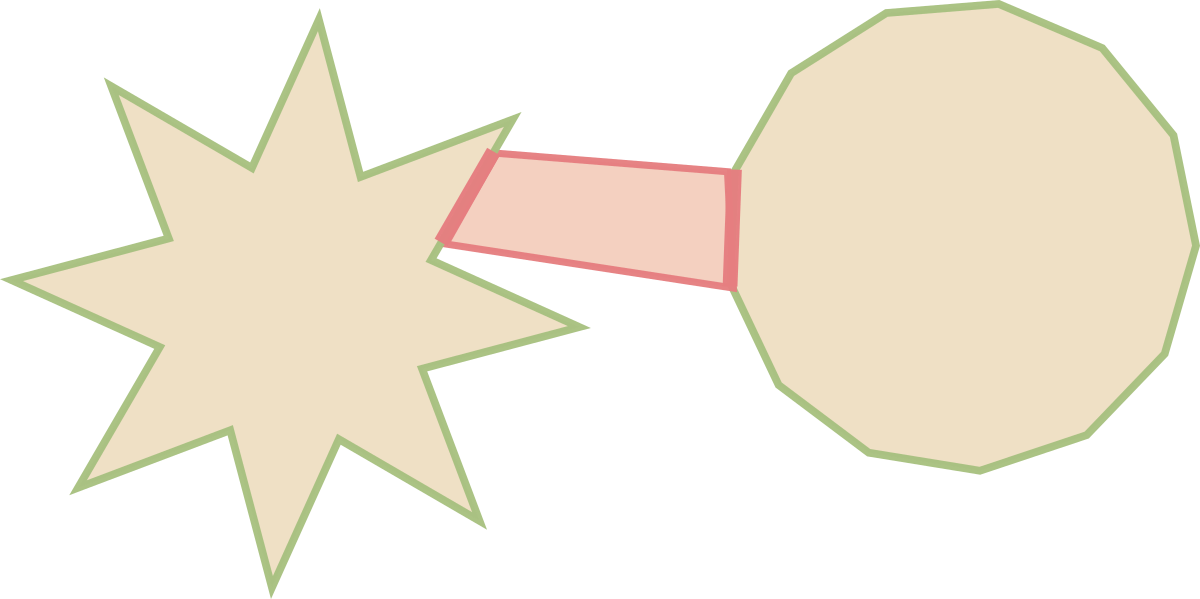
\includegraphics[width=0.6\textwidth]{suma-spojna-powierzchni.png}
  \end{center}

  $$\chi(F_1\# F_2)=\chi(F_1)+\chi(F_2)+\chi(\kwadracik)-2\cdot \chi(\kreska)$$
  $$2-2g(F_1\# F_2)-1=2-2g(F_1)-1+2-2g(F_2)-1+1-2$$
  $$\color{blue}g(F_1\# F_2)=g(F_1)+g(F_2)$$
\end{frame}


\begin{frame}{Powierzchnie orientowalne}
  Powierzchnia zbudowana z trójkącików jest orientowalna, jeśli 
  \begin{itemize}
    \item możemy wybrać orientację trójkącików taką, że krawędzie współdzielone przez dwa trójkąciki mają dwie strzałki,
    \item lub można narysować strzałeczki w środku każdego i wszystkie zgadzają się lub nie z zegarem
  \end{itemize}

  \begin{center}\scalebox{1.5}{
    \begin{tikzpicture}
      \begin{scope}
        \fill[green!20!bg-dim] (0,0)--(0.5, 1)--(1,0)--(0,0);
        \draw[->, thick](0, 0)--(0.25, 0.5);
        \draw[thick] (0.25, 0.5)--(0.5, 1);
        \draw[->, thick] (0.5, 1)--(0.75, 0.5);
        \draw[thick] (0.75, 0.5)--(1, 0);
        \draw[->, thick] (1, 0)--(0.5, 0);
        \draw[thick] (0.5, 0)--(0, 0);

        \draw (0.5, 0.2) arc (-90:-360:0.1);
        \draw[->] (0.6, 0.25)--(0.6, 0.24);
      \end{scope}

      \begin{scope}[rotate around={180:(0.5, 0.5)}, shift={(0.7, -0.2)}]
        \fill[orange!20!bg-dim] (0,0)--(0.5, 1)--(1,0)--(0,0);
        \draw[->, thick](0, 0)--(0.25, 0.5);
        \draw[thick] (0.25, 0.5)--(0.5, 1);
        \draw[->, thick] (0.5, 1)--(0.75, 0.5);
        \draw[thick] (0.75, 0.5)--(1, 0);
        \draw[->, thick] (1, 0)--(0.5, 0);
        \draw[thick] (0.5, 0)--(0, 0);

      \end{scope}
        
      \begin{scope}[shift={(-0.7, 0.6)}]
        \draw (0.5, 0.2) arc (-90:-360:0.1);
        \draw[->] (0.6, 0.25)--(0.6, 0.24);
      \end{scope}

      \begin{scope}[shift={(-1.4, 0)}]
        \fill[green!20!bg-dim] (0,0)--(0.5, 1)--(1,0)--(0,0);
        \draw[->, thick](0, 0)--(0.25, 0.5);
        \draw[thick] (0.25, 0.5)--(0.5, 1);
        \draw[->, thick] (0.5, 1)--(0.75, 0.5);
        \draw[thick] (0.75, 0.5)--(1, 0);
        \draw[->, thick] (1, 0)--(0.5, 0);
        \draw[thick] (0.5, 0)--(0, 0);

        \draw (0.5, 0.2) arc (-90:-360:0.1);
        \draw[->] (0.6, 0.25)--(0.6, 0.24);
      \end{scope}
    \end{tikzpicture}
  }
  \end{center}
\end{frame}
